% YZM5109 Assignment I -- IEEE conference format (pdfLaTeX).
\documentclass[conference]{IEEEtran}
\usepackage{booktabs,graphicx,amsmath,url,xcolor,array}
\usepackage[hidelinks]{hyperref}

\begin{document}
\title{Does One LoRA Run Beat Prompt Engineering?\\A Controlled Study on GSM8K with Qwen2.5-1.5B-Instruct}
\author{\IEEEauthorblockN{Mete Han Y\i lmaz}
\IEEEauthorblockA{Student No.\ 26587026\\YZM5109 Large Language Models, Y\i ld\i z Technical University}}
\maketitle

\begin{abstract}
We test whether a single LoRA fine-tuning run outperforms prompt engineering on grade-school math
(GSM8K) with Qwen2.5-1.5B-Instruct (Option C). Four conditions are evaluated on all 1{,}319 test problems
with identical greedy decoding: zero-shot direct prompting (C1), zero-shot chain-of-thought (C2),
Program-Aided Language modelling (PAL, C3), and a LoRA fine-tune evaluated with the exact C1 prompt (C4).
Zero-shot CoT is best (75.4\% accuracy), 4.5 points above direct prompting (70.9\%, McNemar
$p{=}2.7{\times}10^{-4}$). The fine-tuned model is \emph{worse} than the untouched model (59.6\%, $-11.3$
points, $p{<}10^{-13}$), although it has the highest answer-format validity (99.4\%). Per-item analysis
explains the drop: fine-tuning on the human-written GSM8K solutions shortened the model's reasoning by 56\%,
and the gap to the original model grows from 7 to 21 points as problems get longer, while per-equation
arithmetic accuracy is unchanged.
\end{abstract}

\section{Introduction}
A pretrained LLM can be adapted to a task by changing its inputs (prompting) or its weights (fine-tuning).
Prompting costs nothing at training time but can lengthen every answer. Low-rank adaptation
(LoRA)~\cite{hu2022lora} trains a small fraction of the parameters but needs labelled data and GPU time.
For small \emph{instruction-tuned} models the trade-off is unclear: they are already tuned heavily on
reasoning data, so a short task-specific fine-tune may help, do nothing, or hurt. We answer the question
\emph{does one LoRA fine-tuning run outperform prompting on the original model?} in a controlled setting
where only the adaptation technique varies, and we use the per-item predictions to explain the outcome.
\textbf{Findings:} prompting wins; zero-shot CoT is best; the fine-tuned model loses 11.3 points because it
learned to reason more briefly, which hurts most on long problems.

\section{Dataset, Model, and Methods}
\subsection{Dataset and model}
\textbf{Dataset:} GSM8K (\texttt{openai/gsm8k}, config \texttt{main})~\cite{cobbe2021gsm8k}: grade-school
word problems with a human-written step-by-step solution and one numeric answer. We use the full splits
without subsampling: 7{,}473 training problems (for C4 and nothing else), no validation split, and all
1{,}319 test problems for every condition. No validation split is needed because prompts and
hyperparameters were fixed before any evaluation and were not tuned. Preprocessing removes the calculator
annotations \texttt{<<\ldots>>} from the reference solutions and takes the number after \texttt{\#\#\#\#}
as the gold answer. \textbf{Model:} \texttt{Qwen/Qwen2.5-1.5B-Instruct}~\cite{qwen25}, a 1.56B-parameter
decoder-only transformer, the largest recommended size that trains comfortably on one GPU.

\subsection{Experimental conditions}
All conditions share the system prompt ``You are a helpful assistant.'' and the instruction \emph{End your
response with ``The answer is: $<$number$>$''}, so the output format is held fixed. Exact prompts are in
Appendix~\ref{app:prompts}.
\begin{itemize}
\item \textbf{C1 Zero-shot direct:} the question with a plain ``Solve the following math problem.''
\item \textbf{C2 Zero-shot CoT}~\cite{kojima2022large,wei2022chain}: C1 plus an instruction to reason step
by step, write out every intermediate calculation and check the result.
\item \textbf{C3 PAL}~\cite{gao2023pal}: the model writes a Python function \texttt{solution()}; we execute it
in an isolated subprocess with a 5\,s timeout. Arithmetic is delegated to the interpreter.
\item \textbf{C4 LoRA:} the original model fine-tuned once and evaluated with the \emph{identical} C1 prompt.
Prompting techniques are not re-applied to C4.
\end{itemize}

\subsection{Fine-tuning (C4)}
Inputs are C1 prompts; targets are the cleaned reference solutions followed by ``The answer is: $N$''. The
loss covers response tokens only. LoRA ($r{=}16$, $\alpha{=}32$, dropout 0.05) is applied to all attention
and MLP projections (\texttt{q,k,v,o,gate,up,down}): 18.46M trainable parameters, 1.18\% of the model.
AdamW, learning rate $2{\times}10^{-4}$, 5\% warm-up then cosine decay, effective batch 16, 300 steps
(4{,}800 examples, 0.64 epochs, 0.93M tokens), maximum length 512, gradient checkpointing, bf16, seed 42.
Training took 9.2 minutes on one NVIDIA A100-40GB (Google Colab) with 7.1\,GB peak memory. The loss fell
from about 0.6 to a plateau of about 0.41 within roughly 50 steps.

\subsection{Decoding and answer parsing}
Decoding is identical for all conditions: greedy, at most 512 new tokens, no repetition penalty, batch 128.
For C1, C2 and C4 the prediction is the number after ``The answer is'', falling back to
\texttt{\textbackslash boxed\{\}} and then to the last number. For C3 it is the value of \texttt{solution()},
else the last printed value or the program's final bare expression. Software: PyTorch 2.11,
Transformers 5.22.1, PEFT 0.21.2.

\section{Evaluation Metrics}
\textbf{Accuracy} (primary): the share of test problems whose predicted number equals the reference within
$10^{-4}$. GSM8K has exactly one numeric answer, so exact match is unambiguous and needs no judge model.
We report 95\% bootstrap confidence intervals (10{,}000 resamples) and compare conditions with exact
two-sided McNemar tests~\cite{mcnemar1947}, which suit paired binary outcomes on the same items.
\textbf{Answer validity rate}: the share of outputs that follow the required format, i.e.\ contain ``The
answer is: $<$number$>$''; for PAL, the share of programs that run and return a number. It separates
\emph{failing to give a usable answer} from \emph{giving a wrong answer}, which matters for PAL, whose
programs can crash, and for C4, whose output style fine-tuning changes.
\textbf{Mean generated tokens}: inference cost, since prompting techniques trade accuracy for longer outputs.

\section{Results and Discussion}
\begin{table}[t]\centering
\caption{Results on the GSM8K test set, identical greedy decoding. Valid: answer validity rate.
Tok.: mean generated tokens.}\label{tab:main}
\setlength{\tabcolsep}{3.6pt}
\begin{tabular}{lccccc}\toprule
Condition & $n$ & Acc. (\%) & 95\% CI & Valid (\%) & Tok. \\\midrule
C1 Direct & 1319 & 70.9 & [68.4, 73.3] & 96.5 & 217 \\
C2 CoT    & 1319 & \textbf{75.4} & [73.0, 77.7] & 95.6 & 278 \\
C3 PAL    & 1319 & 59.7 & [57.0, 62.4] & 92.6 & 110 \\
C4 LoRA   & 1319 & 59.6 & [56.9, 62.2] & \textbf{99.4} & 95 \\\bottomrule
\end{tabular}\end{table}

\begin{table}[t]\centering
\caption{Exact McNemar tests for ``X vs.\ Y''. $b$: items only X solves; $c$: items only Y solves.}\label{tab:mcnemar}
\begin{tabular}{lcccc}\toprule
Comparison & $\Delta$Acc. (pts) & $b$ & $c$ & $p$ \\\midrule
C2 vs.\ C1 & $+4.5$  & 157 & 98  & $2.7{\times}10^{-4}$ \\
C3 vs.\ C1 & $-11.2$ & 127 & 275 & $1.2{\times}10^{-13}$ \\
C4 vs.\ C1 & $-11.3$ & 114 & 263 & $1.1{\times}10^{-14}$ \\
C4 vs.\ C2 & $-15.8$ & 89  & 297 & $2.9{\times}10^{-27}$ \\
C4 vs.\ C3 & $-0.1$  & 200 & 201 & $1.0$ \\\bottomrule
\end{tabular}\end{table}

\textbf{Overview.} Table~\ref{tab:main} gives the ranking C2 $>$ C1 $>$ C3 $\approx$ C4; all differences are
significant except C3 vs.\ C4 (Table~\ref{tab:mcnemar}). Explicit CoT gains 4.5 points at 28\% more
tokens. The fine-tuned model loses 11.3 points to the model it was trained from, while being the most
format-compliant condition: fine-tuning taught the format but not better reasoning. On cost, prompting needs
no training. C4 needed 9.2 minutes of A100 time, and its unmerged adapters made it slower per item
(0.27\,s vs.\ 0.17\,s for C1) despite shorter outputs; merging them into the base weights would remove this.

\textbf{Why fine-tuning hurt.} The median C4 answer has 84 tokens against 211 for C1: C4 copied the terse
style of the references (55\% of C1 answers use LaTeX derivations, 0\% of C4 answers). The loss concentrates
on long problems (Fig.~\ref{fig:steps}). The C1$-$C4 gap is 6.7 points for problems with 1--2 reference steps
and 8.6, 10.1, 19.4 and 20.7 points for 3, 4, 5 and 6+ steps. Arithmetic is not the cause: re-evaluating every
equation ``\emph{expression} $=$ \emph{number}'' in the outputs gives similar per-equation error rates for C1
(3.8\%), C2 (3.1\%) and C4 (3.5\%). C4 errors are planning errors with correct arithmetic (Table~\ref{tab:errors}).
Qwen2.5-Instruct was already post-trained heavily on math, and its own derivations are longer and more
careful than the human references, so supervised fine-tuning on them imitates a weaker teacher. The low
initial loss and early plateau suggest that more steps would not help. Training on the model's own verified
solutions (rejection-sampling fine-tuning, STaR~\cite{zelikman2022star,yuan2023scaling}) is the natural fix.

\begin{figure}[t]\centering
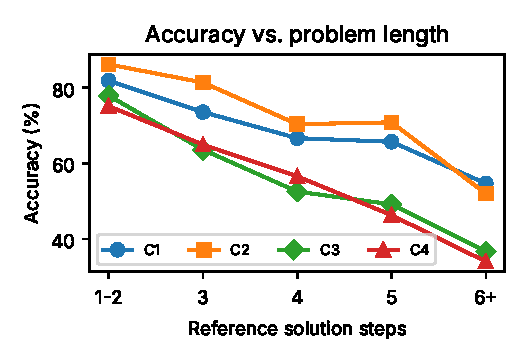
\includegraphics[width=0.9\linewidth]{fig_steps.pdf}
\caption{Accuracy by number of steps in the reference solution (bucket sizes 326, 371, 297, 175, 150).}\label{fig:steps}
\end{figure}

\textbf{Why PAL did not help.} PAL removes arithmetic errors, but at about 3\% per equation there are few to
remove. Its own failures are larger. 7.4\% of programs gave no answer: 85 ended with an assignment instead of
the requested \texttt{solution()} function, 12 raised errors, and none timed out. Only 64.4\% of executable
programs were correct, because turning a word problem into code is itself a reasoning step. As a sensitivity
check, \emph{not} our primary metric, reading the last assigned variable of those 85 programs raises PAL to
64.1\%, still 6.8 points below C1.

\textbf{Direct prompting is already implicit CoT.} At 217 tokens, C1 is not answer-only: the
instruction-tuned model reasons step by step unprompted, so explicit CoT adds structure on top of existing
reasoning and the gain is moderate.

\textbf{Complementarity.} 88.2\% of problems are solved by at least one condition but only 38.1\% by all four.
When CoT and PAL agree (56.8\% of items) the answer is correct 93.6\% of the time, against 51.4\% CoT accuracy
on the rest, a cheap confidence signal for deciding when to trust an answer.

\begin{table}[t]\centering
\caption{Error examples from the test set (sample ID = test-split index).}\label{tab:errors}
\footnotesize\setlength{\tabcolsep}{2.5pt}
\begin{tabular}{@{}l>{\raggedright\arraybackslash}p{0.50\linewidth}c>{\raggedright\arraybackslash}p{0.17\linewidth}@{}}\toprule
ID/Cond. & Problem (abridged) and model behaviour & Gold/Pred. & Failure type \\\midrule
506/C2 & 6 dogs, 4 legs each, snowshoes sold in pairs at \$12. Treats a pair as covering 4 legs. & 144/72 & World-knowledge misreading \\
1018/C2 & 10 min per 3 pages, reads 18 pages. Computes pages/min and multiplies by pages. & 60/5.4 & Inverted rate (units) \\
309/C4 & Extra arm every 3 days, extra leg every 5 days, 15 days. Counts only the arms. & 8/5 & Dropped constraint \\
988/C4 & Saves \$500/month, shoes cost \$1{,}000. Computes ``2 pairs per month''. & 6/24 & Inverted ratio \\
1293/C3 & 5000 bars/day at \$2, two weeks. Correct code, but ends with an assignment and returns nothing. & 140000/-- & Format non-compliance \\\bottomrule
\end{tabular}\end{table}

\section{Conclusion}
A single LoRA run on GSM8K reference solutions did \emph{not} outperform prompting: it lost 11.3 points to
direct prompting and 15.8 points to zero-shot CoT, both highly significant. The failure traces to the
training targets, not to LoRA: fine-tuning taught the model to reason more briefly, which hurts most on long
problems. For this model and task, zero-shot CoT is the best option tested. \textbf{Limitations:} one model,
one seed and one LoRA configuration, so seed variance and the effect of rank or learning rate are not
measured. GSM8K may overlap the model's post-training data. Greedy decoding excludes self-consistency. The
arithmetic checker only parses explicit numeric equations. Latency depends on batch composition.

\section*{Code and AI Usage}
Code, notebook, predictions and the analysis script:
\url{https://github.com/MeteHanYilmaz0/Data_Ai/tree/ccr-36b08569-obh9ku/YZM5109_Assignment1}.
An AI assistant (Claude) was used to design and implement the code, run the post-hoc analysis and draft this
report. The author ran all experiments on Google Colab and reviewed the code, results and text. Details are in
the attached AI usage log.

\begin{thebibliography}{10}
\bibitem{hu2022lora} E.~J. Hu \emph{et al.}, ``LoRA: Low-rank adaptation of large language models,'' in \emph{Proc. ICLR}, 2022.
\bibitem{qwen25} Qwen Team, ``Qwen2.5 technical report,'' \emph{arXiv:2412.15115}, 2024.
\bibitem{cobbe2021gsm8k} K.~Cobbe \emph{et al.}, ``Training verifiers to solve math word problems,'' \emph{arXiv:2110.14168}, 2021.
\bibitem{wei2022chain} J.~Wei \emph{et al.}, ``Chain-of-thought prompting elicits reasoning in large language models,'' in \emph{Proc. NeurIPS}, 2022.
\bibitem{kojima2022large} T.~Kojima \emph{et al.}, ``Large language models are zero-shot reasoners,'' in \emph{Proc. NeurIPS}, 2022.
\bibitem{gao2023pal} L.~Gao \emph{et al.}, ``PAL: Program-aided language models,'' in \emph{Proc. ICML}, 2023.
\bibitem{zelikman2022star} E.~Zelikman, Y.~Wu, J.~Mu, and N.~D. Goodman, ``STaR: Bootstrapping reasoning with reasoning,'' in \emph{Proc. NeurIPS}, 2022.
\bibitem{yuan2023scaling} Z.~Yuan \emph{et al.}, ``Scaling relationship on learning mathematical reasoning with large language models,'' \emph{arXiv:2308.01825}, 2023.
\bibitem{mcnemar1947} Q.~McNemar, ``Note on the sampling error of the difference between correlated proportions or percentages,'' \emph{Psychometrika}, vol.~12, no.~2, pp.~153--157, 1947.
\end{thebibliography}

\appendices
\section{Exact Prompts}\label{app:prompts}
\footnotesize
\textbf{System (all conditions):} \texttt{You are a helpful assistant.}

\textbf{C1 direct (also C4 evaluation and C4 training input):}\\
\texttt{Solve the following math problem.\textbackslash n\textbackslash nQuestion: \{question\}\textbackslash n\textbackslash nEnd your response with "The answer is: <number>".}

\textbf{C2 zero-shot CoT:}\\
\texttt{Solve the following math problem. Let's think step by step: break the problem into smaller steps,
write out every intermediate calculation, and check the result before answering.\textbackslash n\textbackslash nQuestion:
\{question\}\textbackslash n\textbackslash nEnd your response with "The answer is: <number>".}

\textbf{C3 PAL:}\\
\texttt{Write a Python function named `solution()` that solves the following math problem and returns the
final numeric answer. Use descriptive variable names and simple arithmetic. Do not use input() or external
libraries. Reply with a single \`{}\`{}\`{}python code block only.\textbackslash n\textbackslash nQuestion: \{question\}}

\textbf{C4 training target:} \texttt{\{reference solution without <<...>>\}\textbackslash nThe answer is: \{gold\}}
\end{document}
